%\documentclass{article}
%\usepackage{graphicx}
%
%\begin{document}

%\noindent [source] %{\scriptsize https://hub.salford.ac.uk/sirc-acoustics/psychoacoustics/sound-quality-making-products-sound-better/an-introduction-to-sound-quality-testing/roughness-fluctuation-strength/}
%\href{https://hub.salford.ac.uk/sirc-acoustics/psychoacoustics/sound-quality-making-products-sound-better/an-introduction-to-sound-quality-testing/roughness-fluctuation-strength/}{\texttt{\scriptsize https://hub.salford.ac.uk/sirc-acoustics/psychoacoustics/sound-quality-making-prod\\ ucts-sound-better/an-introduction-to-sound-quality-testing/roughness-fluctuation-strength/}}
%
\subsection*{Roughness -- fluctuation
strength}\label{roughness-fluctuation-strength}

Roughness is a complex effect which quantifies the subjective perception
of rapid (15-300 Hz) amplitude modulation of a sound. It is hard to
describe in words, but below are some sound files that hoepfully will
give a sense of what is meant by rapid modulation. The unit of measure
is the asper. One asper is defined as the roughness produced by a 1000Hz
tone of 60dB which is 100\% amplitude modulated at 70Hz {[}1{]}. For a
tone with a frequency of 1000Hz or above, the maximal roughness of a
tone is found to be at a modulating frequency of 70Hz. Maximal roughness
is found to be at increasingly lower modulation frequencies when the
carrier frequency is below 1000Hz. A just noticeable difference level in
roughness is estimated to be 17\% {[}2{]}. Roughness has been used to
partially quantify sound quality in a number of applications including
car engine noise, and in some domestic appliances such as electric
razors. It has also been used in the calculation of an unbiased
annoyance metric.

\begin{figure}[h]
\centering
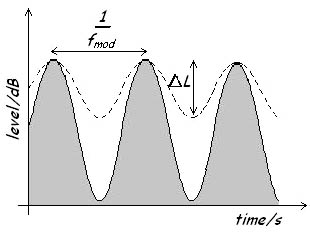
\includegraphics[width=2.525in]{img/model-of-roughness-masking_002.jpg}
\caption*{Figure 1: The effect of subjective duration on rapid amplitude
modulated noise: (i) the modulation depth (unbroken line) and (ii) the
perceived masking depth (dashed line).}
\end{figure}

In order to begin to construct a model for roughness we describe an
amplitude modulated tone as a sound with a rapidly changing loudness
level. To gain understanding of the effect on the ear of this rapidly
changing level we must first understand the concept of subjective
duration.

\subsubsection*{Subjective Duration}\label{subjective-duration}

Usually the duration of a sound refers to the objective duration, and
for sounds greater than 300 ms in length, this is adequate as the
objective measurement and subjective perception are the same. However,
as the duration of a sound gets shorter and goes below 300 ms a
different subjective effect comes into play. Sounds of shorter durations
are perceived to be longer than the objective measurement. For example,
a sound of duration 10ms may be subjectively perceived to be 20 ms long
and this has important consequences for the subjective perception of
temporarily varying sounds, such as rough sounds.

\subsubsection*{How does this relate to
roughness?}\label{how-does-this-relate-to-roughness}

Returning to our amplitude modulated tone we can picture the changing
level of the tone as the unbroken line in figure 1. But because the
duration of a rapidly changing level appears subjectively to be longer,
the level perceived by the ear does not drop as rapidly as the
objectively measured level. So the perceived level only drops as low as
delta L, indicated by the dashed line in figure 1.

\bigskip

To summarise, this means that the perceived masking depth is smaller
than the objectively measured modulation depth. So the roughness of a
sound can be evaluated from the following equation:

\[ R = cal \cdot \int_0^{24Bark}f_{mod} \cdot \Delta L\cdot dz \]


Where $cal$ is a calibration factor, $f_{mod}$ is the frequency of
modulation and $\Delta L$ is the perceived masking depth {[}1{]}.


\begin{figure}[h!]
\centering
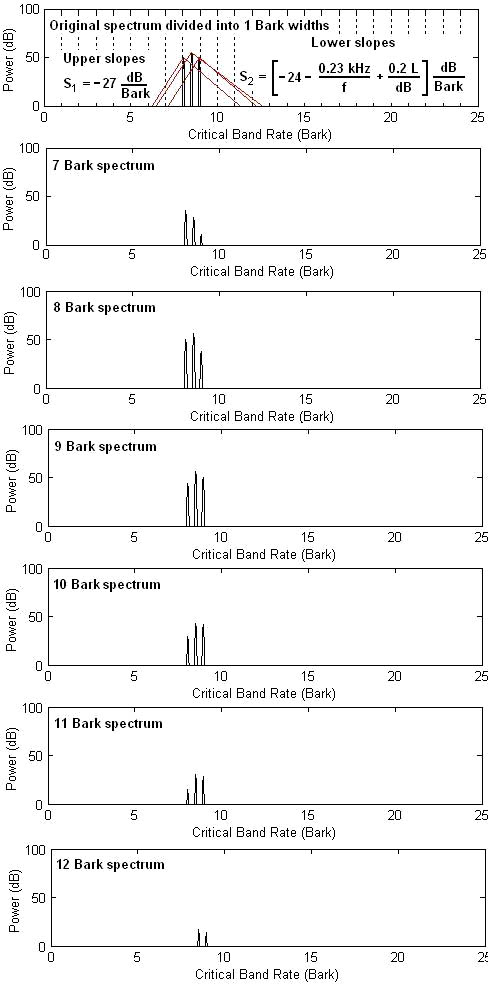
\includegraphics[width=3.225in]{img/roughness-bark-spectrums.jpg}
\caption*{Figure 2: Diagram showing how Bark spectra 7 to 12 are obtained from the
original spectrum.}
\end{figure}

\bigskip

Because of the difficulty in accurately quantifying $\Delta L$, however,
the roughness metric has not yet been standardised and there are several
proposed methods of calculation. One method proposed by Aures {[}3{]} in
1985 requires the calculation of generalised modulation depths
$m^*_i$. First the signal is filtered into 24 individual 1 Bark
wide bands. Next, the envelope of each filtered signal is multiplied by
an appropriate weighting function in the frequency domain that gives
maximal values at 70 Hz (in accordance with the behaviour of roughness).
Then after conversion back to the time domain the r.m.s value of the
each resulting time function is divided by the D.C. value of each
original filtered signal to give 24 generalised modulation depths. These
generalised modulation depths $m^*_i$ are then each multiplied by
a value $g(z_i)$ where $z_i$ is the Bark band of the signal. Each
resulting value $g(z_i) \cdot m^*_i$ is equivalent to $f_{mod}
\cdot \Delta L$ for a particular Bark band so the equation above becomes:

\[ R = cal \cdot \sum_0^{24Bark} g(z_i) \cdot m^*_i \]

Another difficult problem to overcome when developing a roughness
algorithm is to get it to return low values of roughness for random
sound such as white or pink noise. Aures achieved this by using the fact
that the sound was divided up into Bark channels. The filtered spectrum
within each Bark channel can be calculated using slopes devised by
Terhardt {[}6{]} as shown in figure 2.

\bigskip

Calculation of the correlation coefficients between the envelopes of
adjacent Bark bands gives small values for random sounds but large
values if the amplitude modulation in adjacent channels is in phase.
These values can be used to reduce the values of roughness for sounds
such as white noise. Daniel and Weber {[}2{]} develop these ideas
further in their algorithm for calculating roughness.

\bigskip

Widmann \& Fastl {[}4{]} propose another method for calculation, using a
measure of specific loudness made every 2 ms to calculate a time
variable course of the masking pattern and from this a value for $\Delta
L$ can be calculated. Jeong's method {[}5{]} is another proposed method
of calculation.

\subsubsection*{Fluctuation Strength}\label{fluctuation-strength}

Fluctuation strength is similar in principle to roughness except it
quantifies subjective perception of slower (up to 20Hz) amplitude
modulation of a sound. The sensation of fluctuation strength persists up
to 20Hz then at this point the sensation of roughness takes over. There
is a fuzzy border at the change over of the two sensations when it is
difficult to precisely quantify one or the other. 

\bigskip

Fluctuating sound Not fluctuating sound Broad band noise Amplitude
modulated white noise White noise Tonal noise Amplitude modulated 1000
Hz tone 1000 Hz tone

\bigskip

The unit of measure for fluctuation strength is the vacil. One vacil is
defined as the fluctuation strength produced by a 1000Hz tone of 60dB
which is 100\% amplitude modulated at 4Hz. Maximal values are found to
occur at a modulation frequency of 4 Hz. The following relation given by
Fastl {[}1{]} shows the variation of fluctuation strength $F$ with
masking depth $\Delta L$, and modulation frequency $f_{mod}$ :

\[ F = {0.008 \cdot \displaystyle \int_0^{24Bark} \Delta L \cdot dz \over \displaystyle \left({f_{_{mod}} \over 4Hz}\right) + \displaystyle \left({4Hz \over f_{_{mod}}}\right) } \]

It is important to note that $\Delta L$ represents the masking depth.
This is not the same as the modulation depth, in this case, because of
short term memory effects rather than post masking effects. Fluctuation
strength has been used in applications such as to calculate an unbiased
annoyance metric.

\subsubsection*{References}\label{references}

{\small 
\noindent {[}1{]} Zwicker E., Fastl H. \textit{Psychoacoustics: Facts and Models} (1990).

\noindent {[}2{]} P. Daniel and R. Weber, \textit{Psychoacoustic Roughness:
Implementation of an Optimized Model}, Acustica 83, 113$\sim$123 (1997).

\noindent {[}3{]} W. Aures, \textit{Ein Berechnungsverfahren der Rauhigkeit} (`A
Procedure for Calculating Auditory Roughness') Acustica 58, 268$\sim$281 (1985).

\noindent {[}4{]} U. Widmann and H. Fastl, \textit{Calculating roughness using
time-varying specific loudness spectra}, Proc. Sound Quality Symposium 98, 55$\sim$60 (1998).

\noindent {[}5{]} H. Jeong, \textit{Sound quality analysis of nonstationary acoustic
signals}, Ph. D. Thesis, Department of Mechanical Engineering, Korea
Advanced Institute of Science and Technology (KAIST), 1999.

\noindent {[}6{]} E Terhardt \textit{On the perceptions of periodic sound fluctuation
(Roughness)} Acustica 30, 201, (1974).
}

\begin{center}\rule{0.5\linewidth}{0.5pt}\end{center}

%\href{../phylip.html}{\includegraphics{icons/PHYLIP.gif} ... to the PHYLIP home page}

Source:  Sophie Maluski -- University of Salford Manchester 

\href{https://hub.salford.ac.uk/sirc-acoustics/psychoacoustics/sound-quality-making-products-sound-better/an-introduction-to-sound-quality-testing/roughness-fluctuation-strength/}{\texttt{\small https://hub.salford.ac.uk/sirc-acoustics/psychoacoustics/sound-quality-\\ \indent making-products-sound-better/an-introduction-to-sound-quality-testing/\\ \indent roughness-fluctuation-strength/}}
%\end{document}
